\chapter{Introduction}
\label{chap:introduction}
\section{Motivation}
The \acrfull{TIP} development team at Trondheim municipality had a desire for a more agile development process and wanted a continuous deployment setup for their applications. However because of security concerns they concluded that none of the solutions that were offered for- and compatible with their current environment were sensible to implement. This is where the idea for a self-hosted continuous deployment solution came from.

The need for the application product came from security concerns raised by the TIP-team at Trondheim municipality. They have been users of Continuous Integration, and to some degree \acrfull{CD} for a while; but as the scope of their work grew, so did their need for added security and functionality. After careful review they came to the conclusion that the current solution of using Bitbucket pipelines could not be expanded to supply \acrshort{CD} without introducing security risks. Bitbucket pipelines requires the user to expose a management \acrshort{API} to the open internet, which raises security concerns that will be explored in detail in this document.

\section{Research and Hypothesis}
\begin{tabularx}{\linewidth}{X X}
    \epigraph{Developers and businesses avoid \acrshort{CD} out of fear for applications hosted outside their control.}{\textit{Research problem}}
    & \epigraph{Which, if any, security benefits arise from self-hosted \acrshort{CD} solutions, as opposed to cloud-based solutions?}{\textit{Research question}}
\end{tabularx}
As a result of using a self-hosted \acrshort{CD} solution the authors expect to see a reduced risk associated with use of \acrshort{CD}. It is possible that services facing the internet in a cloud-based solution could be internal in a self-hosted solution. If so, each service available to the internet in all likelihood introduces multiple attack vectors to either the host or the user.

In all likelihood some of the services exposed to the internet would need control of high risk infrastructure. A cloud-based Continuous Delivery solution needs the ability to launch and restart applications running in critical environments. In the case of Continuous Deployment even production environments are at risk. If this is the case, trusting the cloud-solution---here a foreign entity---would pose a risk that any security aware user or group should be wary of. Even if the foreign entity is trustworthy they might be a competitor or otherwise unfit to have control over important infrastructure.

\section{cion}
% Introduce what cion is and was at the end of the fall project, reference that report.
To give context to the engineering results the cion application is summarised in this section. cion is a \acrshort{CD} system with two main parts: (1) a website where administrative users can configure the behaviour of cion, and (2) a backend that updates running services in \textit{Docker Swarm}\footnotemark[1] or \textit{Kubernetes}\footnotemark[1] when certain configurable conditions are met. A thorough explanation of the components of cion can be found in the autumn report in appendix \ref{appendix:autumn}.

\begin{figure}[h!]
  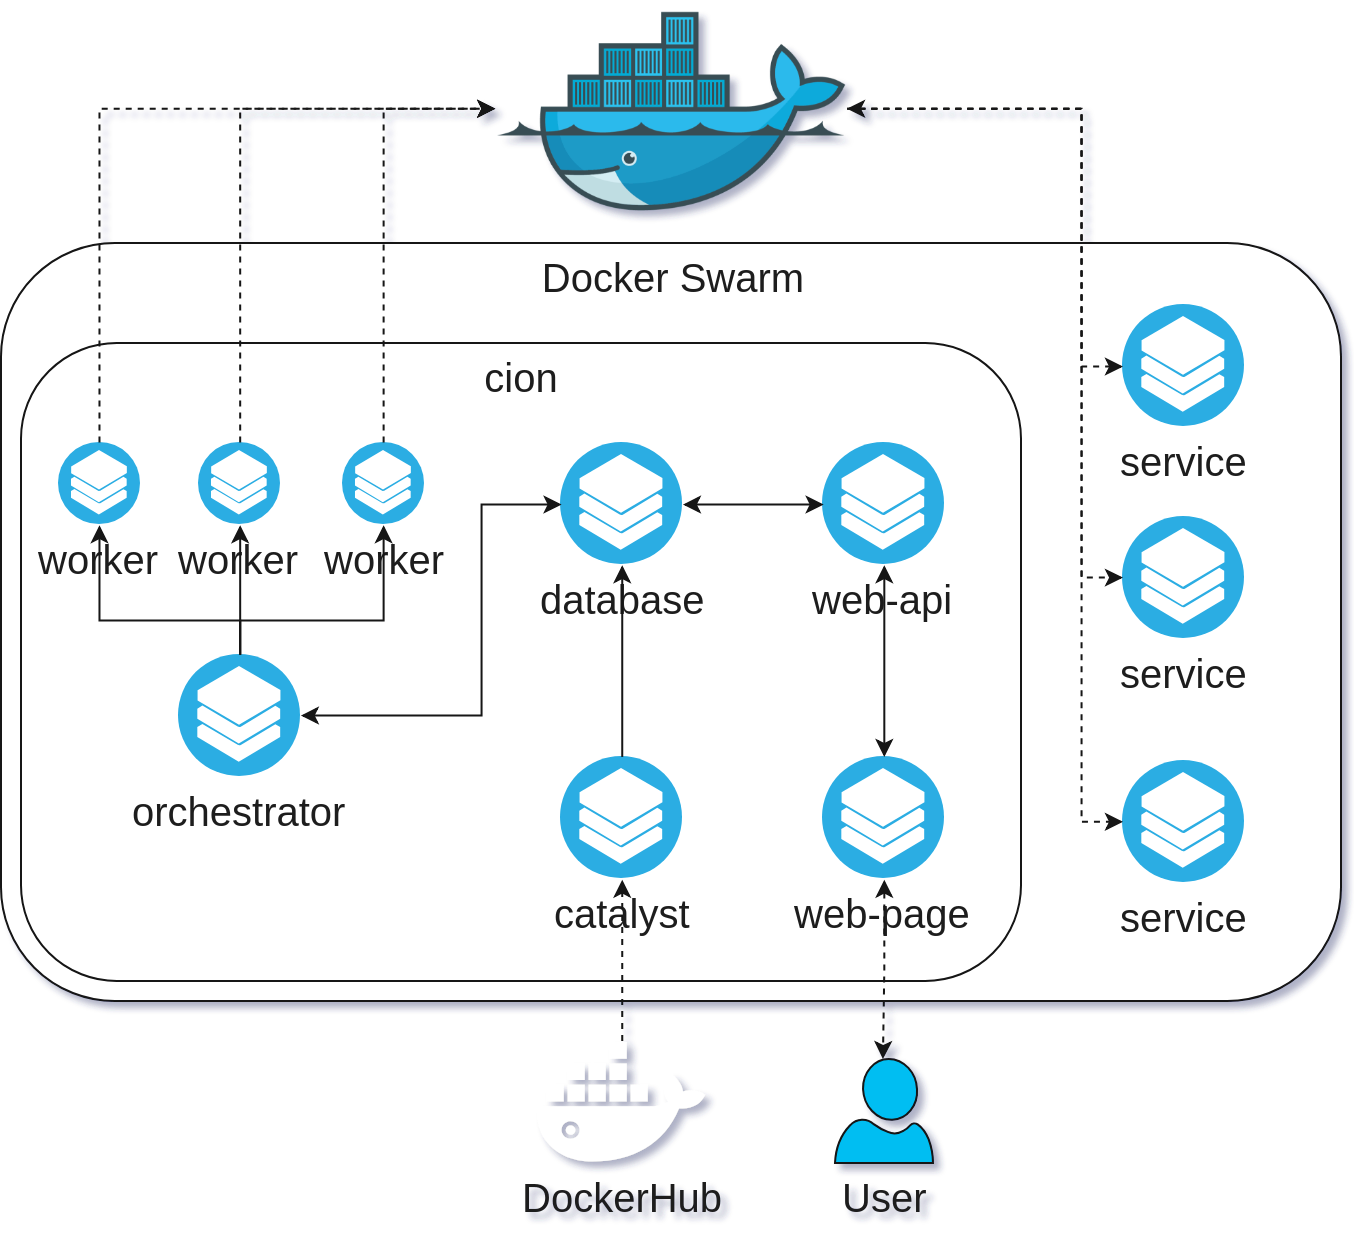
\includegraphics[width=\linewidth,height=\textheight,keepaspectratio]{images/domain_model.png}
  \caption{Application model}
  \label{fig:cionmodel}
\end{figure}

As seen in figure \ref{fig:cionmodel}, cion is composed of a central database that joins the website and the backend. The backend is split into an orchestator service, and a worker service. The orchestrator distributes work to one of the workers. This allows cion to scale up or down the number of workers in response, to changes in workload.

The worker service can perform several different kinds of tasks, however its main task is to update services in \textit{Docker Swarm}\footnotemark[1] and \textit{Kubernetes}\footnotemark[1]. 

The catalyst component listens for external requests to deploy new versions of a service, in figure \ref{fig:cionmodel} the external request is sent by \textit{DockerHub}\footnotemark[1]. \textit{DockerHub}\footnotemark[1] is a \textit{container image host}\footnotemark[1] that can be configured to send \textit{webhooks}\footnotemark[1] whenever a new image is available.

\footnotetext[1]{Explanations of terminology can be found in appendix \ref{appendix:termsexp}}

The cion solution differs from cloud-based and externally hosted \acrshort{CD} solutions in that key components can be hosted in a network physically separate from the internet. In particular the \textit{Docker Swarm} and \textit{Kubernetes} environments' managment \acrshort{API} can be hosted in this manner. The security implications of this is researched in this document.

\section{Report Structure}
\label{sec:reportstructure}
The report is structured into six main chapters that cover larger subjects. The chapters are further divided into multiple subsections. The six main chapters are:

\textbf{\nameref{chap:introduction}} introduces the research question and explains the rest of the report.

\textbf{\nameref{chap:theory}} presents the theoretical background that we base our decisions and work on. 

\textbf{\nameref{chap:process}} explains the technologies used in the software project.

\textbf{\nameref{chap:results}} presents the scientific, engineering and administrative results.

\textbf{\nameref{chap:discussion}} reflects on the results presented in the Results chapter. 

\textbf{\nameref{chap:conclusion}} reflects on how much of the original vision was achieved as well as presents features and changes that could be implemented in the future.

\section{Acronyms and Glossary}
Glossary and acronyms are listed in appendix \ref{appendix:glos} and additional technical terms \& explanations are described in appendix \ref{appendix:termsexp}.
